\subsection{DETER}

Dans le domaine de la cyber-sécurité, le test des solutions de défenses
proposées face aux différentes menaces n'est pas simple et se développe
lentement. En effet, de nombreuses ressources sont nécessaires et il ne semble
pas judicieux d'effectuer les tests en environnement réel. De plus, les
innovations qui fonctionnent parfaitement dans des environnements controllés et
prédictibles sont souvent moins efficaces et fiables dans la réalité de par la
taille du réseau et des ressources qui constituent son environnement. On
ne peut donc pas utiliser la simulation pour tester ces solutions.

Pour être au plus proche de la réalité on va faire de l'émulation, pour cela le
projet DETER \citep{DETER_Project, DETER_benzel2011science,
  DETER_mirkovic2010deter} a été créé. À sa création en 2003, DETER était juste
un projet de recherche avancée visant à développer des méthodes expérimentales
pour les innovations en matière de cyber-sécurité (contrer les cyber-attaques,
trouver les failles réseaux ...). Puis en 2004, le besoin de tester ces méthodes
se faisant de plus en plus sentir, le développement de
DeterLab\footnote{DeterLab: cyber DEfense Technology Experimental Research
  Laboratory} a été lancé. C'est une plateforme d'émulation par interception
libre qui fournit un environnement de test large échelle et réaliste. Elle
permet également d'automatiser et de reproduire des expériences pouvant être de
différentes natures. En effet, DeterlLab peut \textit{i)} observer et analyser
le comportement de cyber-attaques\footnote{ Attaques DDos et botnes, vers et
  codes mallicieux, potocoltes de stockage anti-intrusion (intrusion-tolerant),
  ainsi que le chiffrement et la détection de pattern.} et de technologies de
cyber-défense, \textit{ii)} tester et mesurer l'efficacité des solutions de
défenses proposées pour contrer les menaces. Puisque nous nous intéressons à
l'émulation d'environnements distribués nous allons voir comment fonctionne
l'émulateur DeterLab. Pour fonctionner ce laboratoire viruel a développé 7
outils complémentaires.

Le premier, qui constitue le c\oe ur logiciel et hardware de DeterLab, se base sur
Emulab\footnote{\textbf{todo footnote}} \citep{EMULAB_INIT}, il l'a étendu pour permettre de faire
des tests large échelle spécialisées dans le domaine de la cyber-sécurité et
dont la complexité est représentative des réseaux d'aujourd'hui. Il fournit
également une interface web pour gérer à distance ses expériences, les projets
en développement et accéder aux autres outils de DeterLab.

Pour gérer les ressources nécessaires à leurs expériences les chercheurs du
projet DETER ont créé ``The DeterLab Containers'' (Fig.\ref{Conteneur}). Ces
derniers permettent de virtualiser les ressources et ainsi de répartir la
puissance de calcul là où elle est nécessaire. Ainsi pour des ressources
nécessitant une machine entière le conteneur sera la machine alors que pour une
ressource qui n'aura besoin que d'une partie de la machine, le conteneur sera
une abstraction de cette partie de la machine comme une VM. Cela permet d'isoler
les tests qui n'utilisent pas une machine complète et de partager ses ressources
entre plusieurs tests concurrents. Ce mécanisme de virtualisation s'appelle la
``Multi-resolution Virtualization''.

\begin{figure}
  \centering 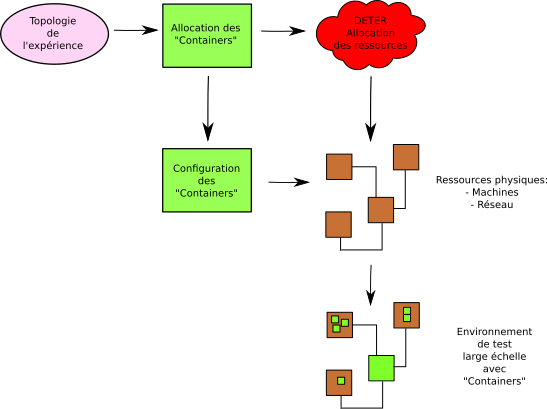
\includegraphics[scale=0.75]{Pictures/png/Deter_fonctionnement_v2}
  \caption{Diagramme du fonctionnement d'un \textit{Container}}
  \label{Conteneur}
\end{figure}

Ensuite, on trouve le simulateur DASH\footnote{Deter Agents
  Simulating Humans} qui permet de prédire le comportement humain en se basant
sur des modèles de pensées, de réactions aux évènements et de comportements
instinctifs ou délibérés.

Dans la réalité, lors de cyber-attaques ou cyber-defenses, chaque partie n'a qu'une
vision partielle du monde. Par exemple, dans le cas d'un système anti-malware, le
système a une vision complète de son réseau local, mais sa vision de la
topologie globale du réseau est partielle. Le système doit donc prendre
en compte ce facteur pour toutes ses actions. Pour intégrer ce facteur à
DeterLab DETER a créé ``Multi-party Experiments''. Cet outil permet de
configurer pour chaque entité d'une expérience le flux d'information qu'elle
difuse et à qui, ainsi que son degré de visibilité sur le réseau.

Afin, construire un environnement de test utilisant des ressources hétérogènes
controllées par leur propriètaire et dont l'usage et les règles de sécurité
d'accès sont différentes le projet DETER a créé la
``Federation''\citep{DETER_faber2007deter}\textbf{to develop?}(Fig.\ref{Federation}).

\begin{figure}
  \centering 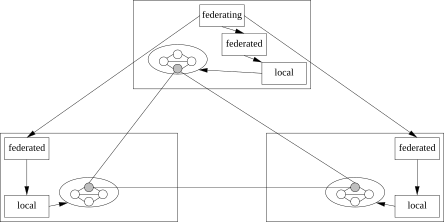
\includegraphics[scale=0.75]{Pictures/png/Deter_federation}
  \caption{Fédération d'une experience réparties sur 3 plateformes de tests différentes}
  \label{Federation}
\end{figure}

MAGI\footnote{Montage AGent Infrastructure} fournit un systèmee de gestion de
flux entre les différentes entités d'une expérience, permettant ainsi d'avoir un
certain contrôle sur les machines. En gérant le flux on peut automatiser et
reproduire les expériences. En effet, MAGI capture chaque séquence
d'instructions concurrentes que l'expérience va suivre pour gérer le flux, ainsi
on peut rejouer la capture plus tard avec les paramètres d'origine ou des
nouveaux si un fichier de paramètres à tester existe. MAGI permet également de
visualiser l'évolution d'une expérience en cours d'exécution pour s'assurer que
son comportement reste correct sans avoir à attendre le résultat final.

Pour finir DETER a créé un dernier outil appelé ``Risky Experiment Management
Capability'' qui permet de controler les expériences ayant besoin d'un accès à
Internet. Pour cela l'outil va placer des portes vers l'extérieur dans
l'infrastructure de l'expérience. Ces portes ne seront pas totalement libres,
pour chaque porte on spécifie le chemin d'entrée et de sortie de
l'infrastructure pour un traffic spécifique et l'adresse de la source ou de la
destination.

 Actuellement, DeterLab peut émuler des dizaines de milliers de n\oe uds. Il est
 le seul émulateur dans le domaine de la cyber-sécurité permettant de faire des
 tests large échelle spécialisées dans le domaine de la cyber-sécurité et dont
 la complexité est représentative des réseaux. \textit{Dernièrement de nouvelles
 expériences sont apparues dans les domaines de la sécurité des réseaux
 avionique et la robustesse de l'anonymat sur le réseau. De plus, des exercices
 et des cours concernant les outils fournis par DeterLab et les méthodes
 expérimentales développées au sein du projet DETER sont mis à disposition des
 enseignants en cyber-sécurité et de leurs étudiants.}\textbf{à mettre ou pas?}
